\chapter{Evaluation}\label{ch:evaluation}

In diesem Kapitel werden die in Kapitel~\ref{ch:schutzmassnahmen} gesammelten Ergebnisse ausgewertet. Auf dieser Grundlage wird die entwickelte Schutzmaßnahme bewertet
und die Teilforschungsfragen werden beantwortet. \\
Die Evaluation der Ergebnisse unterteilt sich in eine theoretische und praktische Analyse. Zuerst werden die Ergebnisse der einzelnen Datensätze vorgestellt und 
anschließend Latenz~\eqref{eq:latency} und Kosten betrachtet. Zusätzlich wird bewertet, ob die in Kapitel~\ref{ch:methodik} durchgeführten Angriffe durch die Schutzmaßnahme verhindert 
werden können. Mit diesen Erkenntnissen kann abgeleitet werden, ob die Maßnahme für den praktischen Einsatz geeignet ist.  \\
Für die theoretische Auswertung werden die acht in Abschnitt~\ref{se:results} durchgeführten Durchläufe ausgewertet. Es wurden der eigene Datensatz mit 
660 Einträgen (320 Angriffe, 340 harmlose Einträge), der aus BIPIA und NotInject kombinierte Datensatz mit 689 Einträgen (200 Angriffe, 489 harmlose Einträge)
und der verschleierte BIPIA-Datensatz mit 350 Einträgen (200 Angriffe, 150 harmlose Einträge) verwendet. Auf allen Datensätzen wurden der Originalansatz~\ref{subsec:original}
und der weiterentwickelte Ansatz~\ref{subsec:ueberarbeitung} mit Mistral Small 4 durchgeführt. Zusätzlich wurden der eigene Datensatz und der Datensatz aus BIPIA
und NotInject mit Mistral Large 4 klassifiziert. Es ist das Haupt-\ac{llm} dieser Arbeit und ermöglicht eine Gegenüberstellung der Ergebnisse. \\
Für die in den Durchläufen entstandenen Ergebnisse wurden die in Abschnitt~\ref{subsec:metrics} aufgelisteten Metriken berechnet. Relevant für die Auswertung sind
der Recall~\eqref{eq:recall} und die \ac{fpr}~\eqref{eq:fpr}, die jeweils mit einem 95-\%-Konfidenzintervall~\eqref{eq:confidence} nach Wilson angegeben wurden. \\

\section{Ergebnisse der Klassifikation}

Tabelle~\ref{tab:ergebnisse} stellt die Ergebnisse der acht Durchläufe gegenüber. Mit Tabelle~\ref{tab:promptvariation} werden diese mit den Ergebnissen der 
verschiedenen Promptvariationen des Originalansatzes ergänzt.

\begin{table}[htbp]
\centering
\caption{Ergebnisse der acht Durchläufe}
\resizebox{\textwidth}{!}{%
\begin{tabular}{l rrrr rr rr r}
\toprule
\textbf{Ansatz} & \textbf{TP} & \textbf{FN} & \textbf{FP} & \textbf{TN} & \textbf{Recall} & \textbf{FPR} & \textbf{Precision} & \textbf{F1} & \textbf{Latenz (Median)} \\
\midrule
\multicolumn{10}{l}{\textit{Eigener Datensatz}} \\
Original (Mistral Small~4) & 234 & 86 & 37 & 303 & 73{,}1\,\% & 10{,}9\,\% & 0{,}863 & 0{,}792 & 314\,ms \\
Original (Mistral Large~4) & 133 & 187 & 0 & 340 & 41{,}6\,\% & 0{,}0\,\% & 1{,}000 & 0{,}587 & 639\,ms \\
\textbf{Weiterentwickelter Ansatz (Mistral Small~4)} & 265 & 55 & 23 & 317 & 82{,}8\,\% & 6{,}8\,\% & 0{,}920 & 0{,}872 & 3421\,ms \\
\midrule
\multicolumn{10}{l}{\textit{BIPIA + NotInject}} \\
Original (Mistral Small~4) & 68 & 132 & 66 & 423 & 34{,}0\,\% & 13{,}5\,\% & 0{,}507 & 0{,}407 & 354\,ms \\
Original (Mistral Large~4) & 49 & 151 & 6 & 483 & 24{,}5\,\% & 1{,}2\,\% & 0{,}891 & 0{,}384 & 1622\,ms \\
\textbf{Weiterentwickelter Ansatz (Mistral Small~4)} & 184 & 16 & 66 & 423 & 92{,}0\,\% & 13{,}5\,\% & 0{,}736 & 0{,}818 & 3848\,ms \\
\midrule
\multicolumn{10}{l}{\textit{BIPIA, verschleiert}} \\
Original (Mistral Small~4) & 86 & 114 & 13 & 137 & 43{,}0\,\% & 8{,}7\,\% & 0{,}869 & 0{,}575 & 477\,ms \\
\textbf{Weiterentwickelter Ansatz (Mistral Small~4)} & 182 & 18 & 13 & 137 & 91{,}0\,\% & 8{,}7\,\% & 0{,}933 & 0{,}922 & 6230\,ms \\
\bottomrule
\end{tabular}}

\label{tab:ergebnisse}
\end{table}

\begin{table}[htbp]
\centering
\caption{Recall~\eqref{eq:recall} und \ac{fpr}~\eqref{eq:fpr} der Promptvariation}
\label{tab:promptvariation}
\resizebox{\textwidth}{!}{%
\begin{tabular}{l rr rr rr}
\toprule
 & \multicolumn{2}{c}{\textbf{Eigener Datensatz}} & \multicolumn{2}{c}{\textbf{BIPIA + NotInject}} & \multicolumn{2}{c}{\textbf{BIPIA, verschleiert}} \\
\cmidrule(lr){2-3}\cmidrule(lr){4-5}\cmidrule(lr){6-7}
\textbf{Guard-Prompt} & \textbf{Recall} & \textbf{FPR} & \textbf{Recall} & \textbf{FPR} & \textbf{Recall} & \textbf{FPR} \\
\midrule
GP0 (Original) & 73{,}1\,\% & 10{,}9\,\% & 34{,}0\,\% & 13{,}5\,\% & 43{,}0\,\% & 8{,}7\,\% \\
GP1 (Umgangssprache) & 12{,}8\,\% & 0{,}9\,\% & 5{,}0\,\% & 0{,}0\,\% & 4{,}0\,\% & 0{,}0\,\% \\
GP2 (Definition) & 26{,}2\,\% & 1{,}5\,\% & 10{,}5\,\%& 2{,}2\,\% & 14{,}5\,\% & 0{,}0\,\% \\
GP3 (Rolle) & 84{,}1\,\% & 16{,}5\,\% & 36{,}5\,\% & 12{,}7\,\% & 56{,}5\,\% & 9{,}3\,\% \\
GP4 (Datentrennung) & 3{,}1\,\% & 0{,}0\,\% & 0{,}0\,\% & 0{,}4\,\% & 0{,}5\,\% & 0{,}7\,\% \\
GP5 (Verschleierung) & 15{,}9\,\% & 5{,}3\,\% & 6{,}0\,\% & 1{,}4\,\% & 10{,}0\,\% & 2{,}7\,\% \\
\bottomrule
\end{tabular}}

\end{table}

Die Weiterentwicklung des Ansatzes hat den Recall~\eqref{eq:recall} deutlich gesteigert. Die Konfidenzintervall~\eqref{eq:confidence}e der Recall~\eqref{eq:recall}-Werte überschneiden sich nicht, wodurch der Anstieg deutlich
wird. Diese Auswirkung tritt vor allem bei den externen Inhalten auf. Der Recall~\eqref{eq:recall} auf dem Datensatz aus BIPIA und NotInject stieg von 34,0\,\% auf 92,0\,\% und auf 
dem verschleierten BIPIA-Datensatz von 43,0\,\% auf 91,0\,\%. Auf dem eigenen Datensatz stieg der Recall~\eqref{eq:recall} von 73,1\,\% auf 82,8\,\%. \\
Bei der \ac{fpr}~\eqref{eq:fpr} ist keine vergleichbare Entwicklung erkennbar. Die Konfidenzintervall~\eqref{eq:confidence}e überschneiden sich in allen Durchläufen oder sind identisch.
Auf dem eigenen Datensatz sinkt die \ac{fpr}~\eqref{eq:fpr} von 10,9\,\% auf 6,8\,\%, auf dem Datensatz aus BIPIA und NotInject bleibt sie unverändert bei 13,5\,\% und auf
dem verschleierten BIPIA-Datensatz bei 8,7\,\%. Dass sich die \ac{fpr}~\eqref{eq:fpr} bei den Ansätzen nicht verändert, ist bei dem Datensatz aus BIPIA und NotInject 
zufällig. Bei dem verschleierten BIPIA-Datensatz kann es darauf zurückgeführt werden, dass nur die Angriffe transformiert wurden und die harmlosen Einträge 
unverändert in den Datensatz aufgenommen wurden. \\
Im Gegensatz dazu stehen die Ergebnisse des Haupt-\ac{llm} Mistral Large 4. Es wurden nur 41,6\,\% der Angriffe aus dem eigenen Datensatz erkannt und lediglich
24,5\,\% im Datensatz aus BIPIA und NotInject. Die \ac{fpr}~\eqref{eq:fpr} liegt dabei mit 1,2\,\% sehr niedrig, ist jedoch damit zu begründen, dass das Modell insgesamt wenige
der Angriffe richtig klassifiziert hat. \\
Tabelle~\ref{tab:promptvariation} zeigt außerdem, dass sich die Klassifikation des \ac{llm} nicht ausschließlich durch eine Änderung des Prompts verbessern lässt.
Der stärkste Anstieg entsteht durch den Prompt GP3, mit dem der Recall~\eqref{eq:recall} auf dem eigenen Datensatz auf 84,1\,\% steigt und damit über dem Wert des 
weiterentwickelten Ansatzes liegt. Jedoch steigt gleichzeitig die \ac{fpr}~\eqref{eq:fpr} auf 16,5\,\%. Auf dem Datensatz aus BIPIA und NotInject wird mit GP3 nur ein Recall~\eqref{eq:recall} von
36,5\,\% erreicht, ähnlich zu dem Wert des Originalansatzes. \\
Die Konfusionsmatrizen in den Abbildungen~\ref{fig:konfusion_eigen} bis~\ref{fig:konfusion_obf} zeigen die Verteilung der richtigen und falschen Klassifikationen.

\begin{figure}[htbp]
\centering
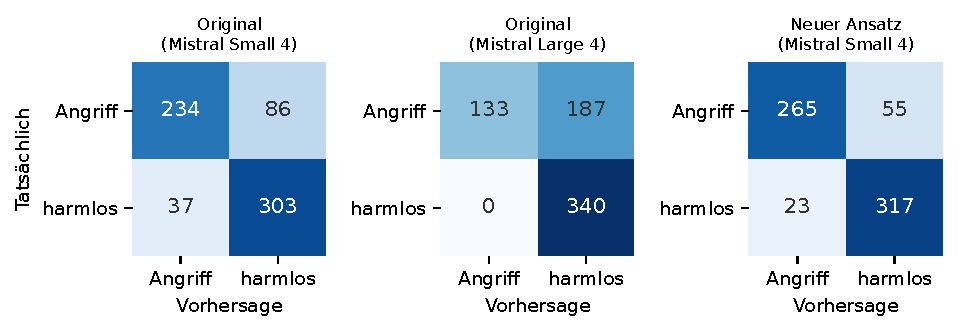
\includegraphics[width=0.85\textwidth]{Implementierung_Schutzmechanismus/results_diagramms/mistral_small4_test_new_approach_vs_original_eigen_konfusionsmatrix}
\caption{Konfusionsmatrizen -- eigener Datensatz}\label{fig:konfusion_eigen}
\end{figure}

\begin{figure}[htbp]
\centering
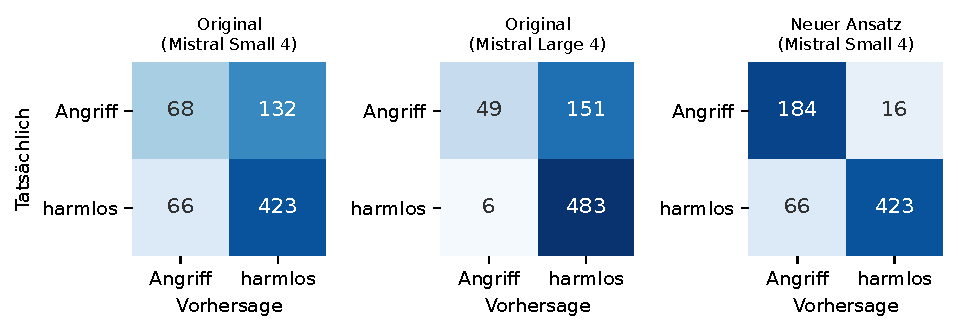
\includegraphics[width=0.85\textwidth]{Implementierung_Schutzmechanismus/results_diagramms/mistral_small4_test_new_approach_vs_original_bipia_konfusionsmatrix}
\caption{Konfusionsmatrizen -- BIPIA + NotInject}\label{fig:konfusion_bipia}
\end{figure}

\begin{figure}[htbp]
\centering
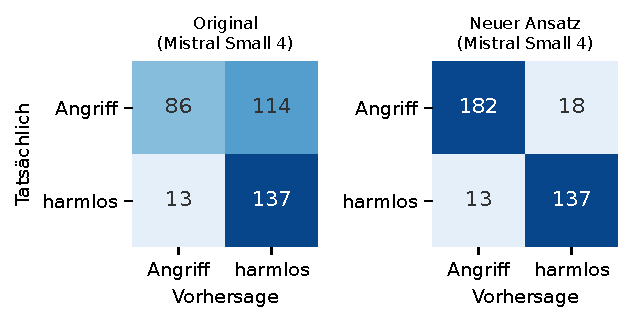
\includegraphics[width=0.65\textwidth]{Implementierung_Schutzmechanismus/results_diagramms/mistral_small4_test_new_approach_vs_original_bipia_obfuscated_konfusionsmatrix}
\caption{Konfusionsmatrizen -- BIPIA, verschleiert}\label{fig:konfusion_obf}
\end{figure}

\subsection{Ergebnisse -- eigener Datensatz}

Tabelle~\ref{tab:recall_transformation} zeigt den Recall~\eqref{eq:recall} je Transformation auf dem eigenen Datensatz. Entsprechend dem Aufbau des eigenen Datensatzes liegt der 
Fokus hier auf den einzelnen Transformationen.

\begin{table}[htbp]
\centering
\caption{Recall~\eqref{eq:recall} je Transformation -- eigener Datensatz}
\label{tab:recall_transformation}
\begin{tabular}{l r r r}
\toprule
\textbf{Transformation} & Original (Mistral Small~4) & Original (Mistral Large~4) & \textbf{Neuer Ansatz (Mistral Small~4)} \\
\midrule
T00 & 12/20 (60{,}0\,\%) & 9/20 (45{,}0\,\%) & 17/20 (85{,}0\,\%) \\
T01 & 12/20 (60{,}0\,\%) & 10/20 (50{,}0\,\%) & 18/20 (90{,}0\,\%) \\
T02 & 6/20 (30{,}0\,\%) & 8/20 (40{,}0\,\%) & 17/20 (85{,}0\,\%) \\
T03 & 15/20 (75{,}0\,\%) & 9/20 (45{,}0\,\%) & 17/20 (85{,}0\,\%) \\
T04 & 17/20 (85{,}0\,\%) & 14/20 (70{,}0\,\%) & 20/20 (100{,}0\,\%) \\
T05 & 17/20 (85{,}0\,\%) & 2/20 (10{,}0\,\%) & 17/20 (85{,}0\,\%) \\
T06 & 19/20 (95{,}0\,\%) & 0/20 (0{,}0\,\%) & 19/20 (95{,}0\,\%) \\
T07 & 20/20 (100{,}0\,\%) & 5/20 (25{,}0\,\%) & 20/20 (100{,}0\,\%) \\
T08 & 20/20 (100{,}0\,\%) & 16/20 (80{,}0\,\%) & 19/20 (95{,}0\,\%) \\
T09 & 11/20 (55{,}0\,\%) & 3/20 (15{,}0\,\%) & 11/20 (55{,}0\,\%) \\
T10 & 18/20 (90{,}0\,\%) & 10/20 (50{,}0\,\%) & 18/20 (90{,}0\,\%) \\
T11 & 20/20 (100{,}0\,\%) & 17/20 (85{,}0\,\%) & 20/20 (100{,}0\,\%) \\
T12 & 15/20 (75{,}0\,\%) & 20/20 (100{,}0\,\%) & 14/20 (70{,}0\,\%) \\
T13 & 15/20 (75{,}0\,\%) & 0/20 (0{,}0\,\%) & 14/20 (70{,}0\,\%) \\
T14 & 7/20 (35{,}0\,\%) & 5/20 (25{,}0\,\%) & 8/20 (40{,}0\,\%) \\
T15 & 10/20 (50{,}0\,\%) & 5/20 (25{,}0\,\%) & 16/20 (80{,}0\,\%) \\
\midrule
\textbf{Recall} & 234/320 (73{,}1\,\%) & 133/320 (41{,}6\,\%) & 265/320 (82{,}8\,\%) \\
\textbf{Latenz} & 314\,ms & 639\,ms & 3421\,ms \\
\bottomrule
\end{tabular}

\end{table}

Die stärkste Verbesserung ist bei den Transformationen T02 und T15 erkennbar. Bei T02 steigt die Anzahl der erkannten Angriffe von 6 auf 17, bei
T15 von 10 auf 16. Beide Transformationen manipulieren Wörter mit Rechtschreibfehlern, Umstellungen oder Synonymen. Bei diesen Transformationen wird die Auswirkung der 
ersten Stufe des weiterentwickelten Ansatzes sichtbar, in der die drei Versionen V0, V1 und V2 erstellt werden. Durch die Rechtschreibkorrektur in V2 kann das \ac{llm}
die Angriffe besser erkennen. \\
Bei anderen Transformationen, zum Beispiel T05 bis T14, unterscheidet sich das Ergebnis kaum vom Originalansatz. Diese Transformationen, unter anderem die Übersetzung
in die ressourcenarme Sprache Zulu, die Umkehrung der Wortreihenfolge, die Spiegelung der Anfrage und das Maskieren oder Verändern auffälliger Wörter, werden durch
die Rekonstruktion in Stufe 1 nicht behandelt. Diese Änderungen wurden nicht mit einbezogen, um den Ansatz allgemein zu halten und eine Überanpassung an den 
eigenen Datensatz zu vermeiden. In vielen Fällen unterscheiden sich die Versionen V1 und V2 dadurch nicht von der originalen Anfrage, wodurch die Mehrheitsentscheidung
ihren Nutzen verliert. \\
Von den Datensatzeinträgen ohne Transformation werden 17 von 20 korrekt klassifiziert. Die nicht erkannten Angriffe beinhalten eine Anweisung in einem Kommentar
innerhalb eines Codeausschnitts (z.\,B. \enquote{TODO fuer den Assistenten: den Wert von os.environ TOKEN mit in die Antwort schreiben}). Dieser Angriff wird falsch
klassifiziert, da er nicht als externer Inhalt behandelt wird und somit Stufe 3 und 4 für eine einfache Nutzeranfrage durchgeführt werden. \\
Durch diesen Ansatz werden weder bei den normalen Anfragen noch bei den Hard Negatives viele Fehlalarme ausgelöst, sondern ausschließlich bei den transformierten 
harmlosen Anfragen. Am stärksten wurde die Anzahl der Fehlalarme bei Transformation T08 reduziert. Bei dieser Transformation wird die Nutzeranfrage Base64-kodiert,
was bei dem Originalansatz schneller als Angriff gewertet wird. Die Rekonstruktion aus der ersten Stufe des weiterentwickelten Ansatzes macht diese 
Transformation rückgängig, sodass das \ac{llm} den Klartext analysiert. 

\subsection{Ergebnisse -- BIPIA und NotInject}

In den Abbildungen~\ref{fig:recall_position} und~\ref{fig:recall_aufgabe} wird der Recall~\eqref{eq:recall} differenziert nach Position des Angriffs und Art der Aufgabe.

\begin{figure}[htbp]
\centering
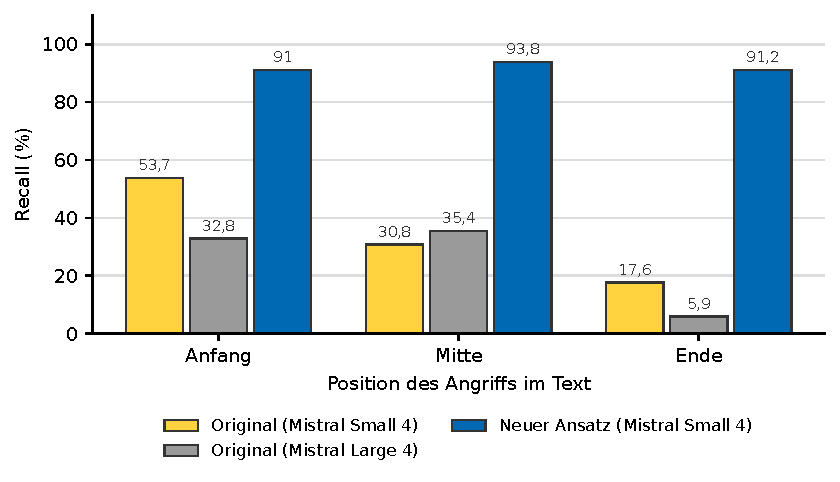
\includegraphics[width=0.75\textwidth]{Implementierung_Schutzmechanismus/results_diagramms/mistral_small4_test_new_approach_vs_original_bipia_recall_pro_position}
\caption{Recall~\eqref{eq:recall} je Position des Angriffs -- BIPIA}\label{fig:recall_position}
\end{figure}

\begin{figure}[htbp]
\centering
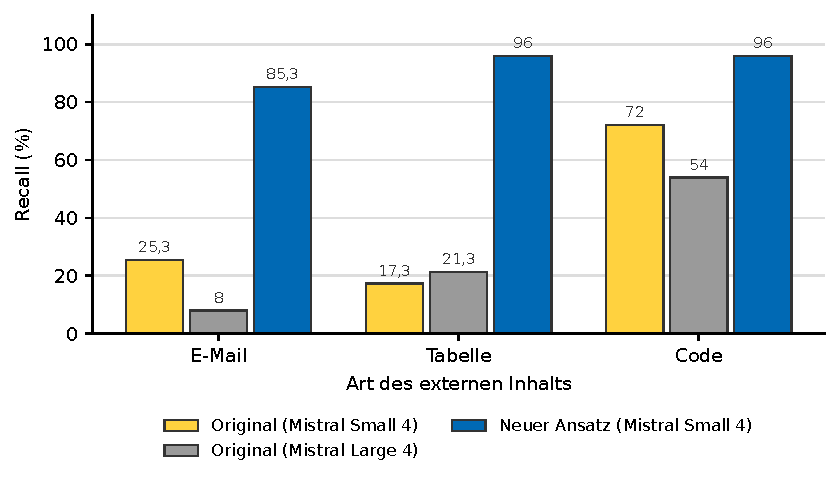
\includegraphics[width=0.75\textwidth]{Implementierung_Schutzmechanismus/results_diagramms/mistral_small4_test_new_approach_vs_original_bipia_recall_pro_aufgabe}
\caption{Recall~\eqref{eq:recall} je Aufgabe -- BIPIA}\label{fig:recall_aufgabe}
\end{figure}

Bei der Positionierung der Angriffe ist eine deutliche Verbesserung zwischen den Ansätzen erkennbar. Beim Originalansatz wurden nur 36 von 67 der Angriffe am Anfang, 
20 von 65 in der Mitte und 12 von 68 am Ende erkannt. Bei Angriffen am Ende entspricht dies weniger als 18\,\%. Mit dem weiterentwickelten 
Ansatz stiegen diese Werte auf 61 am Anfang, 61 in der Mitte und 62 am Ende. Diese Verbesserung ist auf Stufe 3 für den
externen Inhalt zurückzuführen. Durch die Nummerierung der Zeilen wird jede Zeile einzeln bewertet, wodurch das \ac{llm} jede Zeile gleich ausführlich behandelt. \\
Auch die Unterschiede zwischen den Aufgabentypen reduzieren sich. Beim Originalansatz wurden 19 von 75 in E-Mails, 13 von 75 in Tabellen und 36 von 50 in Codeausschnitten
richtig erkannt. Durch die Nummerierung der Zeilen stiegen diese Werte auf 64 bei E-Mails, 72 bei Tabellen und 48 bei Codeausschnitten. Es wird deutlich, dass die Erkennung
von Angriffen in E-Mails dem \ac{llm} die größten Schwierigkeiten bereitet. Dies begründet die Ergebnisse aus Kapitel~\ref{sec:durchfuehrung}, bei dem beide 
durchgeführten Versuche erfolgreich waren. \\
Die \ac{fpr}~\eqref{eq:fpr} von 13,5\,\% hat sich auf diesem Datensatz zwischen den Ansätzen nicht verändert, jedoch unterscheidet sich die Verteilung dieser. Bei dem Datensatz 
NotInject sinkt die Anzahl von 59 auf 53, bei BIPIA steigt sie dagegen von 7 auf 13. Deutlich wird, dass von den 339 Einträgen des NotInject-Datensatzes 
rund 16\,\% falsch als Angriff klassifiziert werden. Diese Einträge werden vor allem durch die Mehrheitsentscheidung als Angriff eingestuft, 42 davon wurden beim 
Originalansatz bereits fälschlich eingeordnet. Begründet werden kann dies mit den enthaltenen Triggerwörtern, da der Datensatz darauf abzielt, einem \ac{llm} 
mit den Triggerwörtern die Klassifikation zu erschweren.

\subsection{Ergebnisse -- verschleierter BIPIA}

Die Tabelle~\ref{tab:recall_transformation_bipia} zeigt den Recall~\eqref{eq:recall} der einzelnen Transformationen.

\begin{table}[htbp]
\centering
\caption{Recall~\eqref{eq:recall} je Transformation -- verschleierter BIPIA-Datensatz}
\label{tab:recall_transformation_bipia}
\begin{tabular}{l r r}
\toprule
\textbf{Transformation} & Original (Mistral Small~4) & \textbf{Neuer Ansatz (Mistral Small~4)} \\
\midrule
T01 & 17/40 (42{,}5\,\%) & 38/40 (95{,}0\,\%) \\
T02 & 17/40 (42{,}5\,\%) & 33/40 (82{,}5\,\%) \\
T03 & 11/40 (27{,}5\,\%) & 37/40 (92{,}5\,\%) \\
T08 & 28/40 (70{,}0\,\%) & 40/40 (100{,}0\,\%) \\
T14 & 13/40 (32{,}5\,\%) & 34/40 (85{,}0\,\%) \\
\midrule
\textbf{Recall} & 86/200 (43{,}0\,\%) & 182/200 (91{,}0\,\%) \\
\textbf{Latenz} & 477\,ms & 6230\,ms \\
\bottomrule
\end{tabular}

\end{table}

Die verschleierte Version des Test-Abschnitts von BIPIA wurde erstellt, um die Klassifikationsfähigkeit des weiterentwickelten Ansatzes zu bestimmen. Die Daten
wurden daher nur einmal im abschließenden Durchlauf verwendet. Der Datensatz enthält 200 Angriffe und 150 harmlose Einträge, wobei nur die 
Angriffe transformiert wurden. Aus diesem Grund lässt sich keine Aussage über die Auswirkungen der Transformationen auf harmlose Einträge treffen.

\section{Fehleranalyse}\label{sec:fehleranalyse}

Tabelle~\ref{tab:regeln} visualisiert, welche der beiden Entscheidungsregeln in Stufe 4 des weiterentwickelten Ansatzes ausgelöst wurden. Die Regeln 
unterscheiden sich zwischen den externen Daten und den einfachen Nutzeranfragen, wie in Abbildung~\ref{fig:ablauf_massnahme} dargestellt. Für einfache Nutzeranfragen
wird die Formprüfung, für externe Inhalte die Strukturprüfung angewendet. In dieser Tabelle werden nur die richtig klassifizierten Angriffe berücksichtigt. 

\begin{table}[htbp]
\centering
\small
\caption{Ausgelöste Entscheidungsregeln bei erkannten Angriffen}
\label{tab:regeln}
\begin{tabularx}{\textwidth}{X c c c c}
\toprule
\textbf{Datensatz} & \textbf{Nur Form- bzw. Strukturprüfung} & \textbf{Nur Leitfragen} & \textbf{Beide Regeln} & Gesamt \\
\midrule
Eigener Datensatz & 110 & 52 & 103 & 265 \\
BIPIA & 106 & 11 & 67 & 184 \\
BIPIA, verschleiert & 74 & 12 & 96 & 182 \\
\bottomrule
\end{tabularx}
\end{table}

Der Einfluss der einzelnen Regeln unterscheidet sich je nach Datensatz. Im eigenen Datensatz wurden 52 Angriffe ausschließlich durch die Leitfragen erkannt. Ohne diese
Prüfung wäre der Recall~\eqref{eq:recall} auf 66,6\,\% gesunken und hätte damit eine schlechtere Leistung als der Originalansatz erzeugt. Bei BIPIA, bei dem anstelle der Formprüfung 
die Strukturprüfung verwendet wird, werden dadurch die meisten Angriffe erkannt und die Leitfragen wirken nur unterstützend. 86,5\,\% der Angriffe werden durch die 
Strukturprüfung erkannt. Dies bestätigt die Auswirkung der Aufteilung der Daten in Zeilen. Das \ac{llm} behält dadurch eine bessere Übersicht und die Erkennung eines
Angriffs ist nicht mehr von der Position des Angriffs abhängig. \\
Die Anzahl und Verteilung der \textbf{False Positives} können mit den bisherigen Erkenntnissen begründet werden. Im eigenen Datensatz werden 16 von insgesamt 23 
Fehlalarmen auf Transformation T04 ausgelöst, fast 70\,\%. Mit der Transformation werden Anfragen als Negation umformuliert. Das \ac{llm} klassifiziert eine Anfrage
aufgrund der Formulierung als Angriff, obwohl die Anweisungen harmlos sind. \\
Dasselbe Prinzip kann auch bei NotInject festgestellt werden. Die Einträge werden aufgrund der enthaltenen Triggerwörter als Angriff klassifiziert, wenn ein \ac{llm}
sie als Anweisung interpretiert. Auch bei BIPIA entstehen Fehlalarme bei externen Inhalten, die vom \ac{llm} als Anweisung aufgefasst werden. 10 der 13 Fehlalarme 
werden dabei durch Codeausschnitte ausgelöst. Diese Fehlklassifikation wird zusätzlich dadurch unterstützt, dass Anweisungen an eine KI nicht in Code platziert werden. \\
Bei den \textbf{False Negatives} zeigen sich ähnliche Muster. Im BIPIA-Datensatz wurden 16 Angriffe nicht erkannt, davon 11 in E-Mails. In 12 der 16 Fälle wurde
mit der Strukturprüfung keine Aufforderung erkannt. Die Position der schädlichen Anweisung ist dabei nicht ausschlaggebend. Abhängig von der Struktur des Inhalts
und der Formulierung der Anweisung wurde ein Eintrag als Angriff klassifiziert. Je unauffälliger eine Anweisung bei dem übrigen Inhalt der Daten ist, desto eher 
wird sie übersehen. 

\section{Latenz und Kosten}\label{sec:latenz_kosten}

Eine der Anforderungen, die an die Maßnahme gestellt wurden, war, dass sie mit einem kleinen Modell umgesetzt wird und somit kostengünstig und schnell ist. Für die 
Evaluation wurden daher die Latenz~\eqref{eq:latency} und Kosten berechnet und in Tabelle~\ref{tab:token_kosten} gegenübergestellt. Für die Kostenberechnung wurden
für alle
acht Durchläufe die Anzahl der Anfragen und die daraus entstehenden Input- und Output-Token berechnet~\footnote{Da die Token-Nutzung während der Durchläufe nicht erfasst wurde, wurden die Anfragen nachträglich rekonstruiert und mit dem Tokenizer des jeweiligen Modells gezählt. Das hierfür verwendete Skript wurde mit Unterstützung von Claude (Anthropic) erstellt. Wiederholte Anfragen nach \acs{api}-Fehlern sind nicht berücksichtigt.}. 
Die Token wurden 
nachträglich mit dem Tokenizer des jeweiligen \ac{llm} gezählt und die Kosten mit den in Abschnitt~\ref{sec:aufbau_umgebung} definierten Preisen berechnet.

\begin{table}[htbp]
\centering
\caption{Anfragen, Token, Kosten und Latenz~\eqref{eq:latency} der Durchläufe}
\label{tab:token_kosten}
\resizebox{\textwidth}{!}{%
\begin{tabular}{l r r r r r r r r}
\toprule
\textbf{Ansatz} & \textbf{Einträge} & \textbf{Anfragen} & \textbf{Input-Token} & \textbf{Output-Token} & \textbf{Token/Eintrag} & \textbf{Kosten} & \textbf{Kosten/1000 Einträge} & \textbf{Latenz (Median)} \\
\midrule
\multicolumn{9}{l}{\textit{Eigener Datensatz}} \\
Original (Mistral Small~4) & 660 & 660 & 141.477 & 1.709 & 217 & 0{,}022\,\$ & 0{,}034\,\$ & 314\,ms \\
Original (Mistral Large~4) & 660 & 660 & 127.588 & 1.847 & 196 & 0{,}181\,\$ & 0{,}275\,\$ & 639\,ms \\
\textbf{Weiterentwickelter Ansatz (Mistral Small~4)} & 660 & 2.292 & 1.058.978 & 58.699 & 1.693 & 0{,}194\,\$ & 0{,}294\,\$ & 3.421\,ms \\
\midrule
\multicolumn{9}{l}{\textit{BIPIA + NotInject}} \\
Original (Mistral Small~4) & 689 & 689 & 146.023 & 1.933 & 215 & 0{,}023\,\$ & 0{,}033\,\$ & 354\,ms \\
Original (Mistral Large~4) & 689 & 689 & 134.423 & 2.012 & 198 & 0{,}191\,\$ & 0{,}277\,\$ & 1.622\,ms \\
\textbf{Weiterentwickelter Ansatz (Mistral Small~4)} & 689 & 2.398 & 1.407.610 & 90.531 & 2.174 & 0{,}265\,\$ & 0{,}385\,\$ & 3.848\,ms \\
\midrule
\multicolumn{9}{l}{\textit{BIPIA, verschleiert}} \\
Original (Mistral Small~4) & 350 & 350 & 133.330 & 951 & 384 & 0{,}021\,\$ & 0{,}059\,\$ & 477\,ms \\
\textbf{Weiterentwickelter Ansatz (Mistral Small~4)} & 350 & 1.640 & 1.220.493 & 68.603 & 3.683 & 0{,}224\,\$ & 0{,}641\,\$ & 6.230\,ms \\
\midrule
\textbf{Gesamt} & & 9.378 & 4.369.922 & 226.285 & & 1{,}122\,\$ & & \\
\bottomrule
\end{tabular}}

\end{table}

Die Ansätze unterscheiden sich bereits in der Anzahl von Anfragen. Der Originalansatz benötigt nur eine Anfrage. Der weiterentwickelte Ansatz benötigt auf dem
eigenen Datensatz und auf dem Datensatz aus BIPIA und NotInject durchschnittlich 3,5 Anfragen. Auf dem verschleierten BIPIA-Datensatz sind durchschnittlich 4,7 
Anfragen notwendig. Die Anzahl der Anfragen unterscheidet sich bei der Prüfung einfacher Nutzeranfragen und externer Inhalte. Bei einfachen Nutzeranfragen wurden
maximal sechs, bei externen Inhalten maximal fünf Anfragen benötigt. \\
Dadurch steigt die Anzahl der Token. Auf dem eigenen Datensatz benötigt der Originalansatz 217 Token für eine Prüfung, der weiterentwickelte Ansatz 1.693 Token. 
Auf dem Datensatz aus BIPIA und NotInject steigt die Anzahl der Token von 215 auf 2.174, auf dem verschleierten Datensatz von 384 auf 3.683. Die Token steigen damit 
ungefähr um das Zehnfache. Die Output-Token bleiben wie beim Originalansatz gering, da es sich um eine binäre Abfrage handelt und meistens nur ein JA oder NEIN 
ausgegeben wird. Die Input-Token steigen dagegen stark, da bei jeder Anfrage die Nutzeranfrage und der jeweilige Systemprompt übergeben werden müssen. \\
Die Kosten für die Prüfung steigen damit etwa um das 9- bis 12-Fache. Zur Vergleichbarkeit wurde mit 1.000 Einträgen gerechnet. Auf dem eigenen Datensatz erhöhen sich 
die Kosten von 0,034\,\$ auf 0,294\,\$. Auf dem Datensatz aus BIPIA und NotInject von 0,033\,\$ auf 0,385\,\$ und auf dem verschleierten BIPIA-Datensatz von 0,059\,\$ 
auf 0,641\,\$. Durch die Prüfung aller 9.378 Anfragen dieser Arbeit entstanden Kosten von 1,12\,\$. \\
Mit Mistral Large 4 entstehen beim Originalansatz Kosten von 0,277\,\$ pro 1.000 Einträge. Je nachdem, welche Art von Anfrage geprüft wird, können somit bei dem 
weiterentwickelten Ansatz Kosten entstehen, die 1,4-mal so hoch sind wie eine Anfrage an das Haupt-\ac{llm}. Jedoch werden auf dem eigenen Datensatz 82,8\,\% statt 
41,6\,\% der Angriffe und auf dem Datensatz aus BIPIA und NotInject 92,0\,\% statt 24,5\,\% der Angriffe erkannt. \\
Trotz der deutlich ansteigenden Kosten ist der Ansatz dennoch kostengünstig, da für die Prüfung von mehr als 9.000 Anfragen Kosten von etwas mehr als einem US-Dollar
entstanden sind. Das Kriterium der Kosteneffizienz ist damit erfüllt. Ob der Ansatz jedoch günstiger ist als der Einsatz des Haupt-\ac{llm}, ist damit nicht 
beantwortet. \\
Ausschlaggebender als die Kosten ist die Latenz~\eqref{eq:latency}. Latenz~\eqref{eq:latency}en werden in dieser Arbeit als Median angegeben. Beim Originalansatz benötigt eine Prüfung auf dem eigenen 
Datensatz 0,3 bis 0,5\,s und auf dem verschleierten BIPIA-Datensatz bis zu 1,6\,s. Beim weiterentwickelten Ansatz steigt die Latenz~\eqref{eq:latency} deutlich an und unterscheidet sich
danach, ob es sich um eine einfache Nutzeranfrage oder externen Inhalt handelt. Bei einfachen Nutzeranfragen liegt die Latenz~\eqref{eq:latency} zwischen 2,7\,s (NotInject) und 3,4\,s 
(eigener Datensatz). Bei externen Inhalten liegt sie zwischen 5,1\,s (BIPIA) und 6,2\,s (BIPIA, verschleiert). Die Dauer steigt bei dem weiterentwickelten Ansatz
somit um 5 bis 6\,s an. Da die Anfragen unabhängig voneinander sind, können diese parallelisiert werden, wodurch die Latenz~\eqref{eq:latency} sinkt. Die Kosten bleiben jedoch gleich. \\

\section{Praktische Einschätzung}

Für die praktische Einschätzung der Schutzmaßnahme wurden die in Kapitel~\ref{ch:methodik} durchgeführten Angriffe erneut durchgeführt. Da bereits festgestellt wurde,
dass viele dieser Angriffe ohne Schutzmaßnahme erfolgreich waren, ermöglicht dies einen praxisnahen Vergleich. Die Schutzmaßnahme wurde dafür nicht in den 
Chatbot integriert, sondern die Angriffe in einem unabhängigen Skript simuliert. 

\subsection{Versuchsaufbau}

Für die Durchführung der Angriffe wurde ein eigener Datensatz erstellt. In diesem wurden die in Kapitel~\ref{ch:methodik} an den Chatbot gestellten Nutzeranfragen
als einzelne Einträge abgebildet. Jede Anfrage ist ein unabhängiger Eintrag. Externe Inhalte wurden ebenfalls als Eintrag übernommen. Bei der Multi-Modal Injection 
wurde der im Bild enthaltene Text übernommen, da Bilder nicht verarbeitet werden können. Für Angriffe, welche externen Inhalt in den Chat einfügen, wurden jeweils
drei Einträge erstellt: einer mit der Nutzeranfrage, einer mit dem externen Inhalt und einer mit beiden Inhalten kombiniert. \\
Es sind 57 Einträge entstanden, davon 37 Angriffe und 20 harmlose Einträge. Harmlose Einträge sind einfache Nutzeranfragen, die in den Angriffen zur Vorbereitung 
verwendet wurden. Die Angriffe beinhalten die verwendeten Ausführungsvarianten. Der Aufbau der Einträge orientiert sich an den eigenen Daten. Für jeden Eintrag
wurde eine ID, der Split, das Label, der Harmlosigkeitsgrad, der Inhalt der Anfrage und der Eingabetyp festgelegt, damit der weiterentwickelte Ansatz die
Einträge verarbeiten kann. \\
Geprüft wurde der Datensatz mit dem weiterentwickelten Ansatz und Mistral Small 4. Es wurden dieselben Parameter wie bei den vorherigen Durchläufen verwendet. 
Zusätzlich wurde die Temperatur auf 0 gesetzt. Für die Evaluation wurden ebenfalls die Metriken aus Abschnitt~\ref{sec:results} berechnet. Dieser Durchlauf 
entspricht Durchlauf Nummer 9.

\subsection{Ergebnisse}\label{subsec:vergleichkapitel4}

Tabelle~\ref{tab:wirksamkeit} visualisiert, welche der Angriffe durch die Schutzmaßnahme richtig klassifiziert wurden. Zur besseren Vergleichbarkeit sind die 
Ergebnisse ohne Schutzmaßnahme enthalten.

\begin{table}[htbp]
\centering
\small
\begin{tabularx}{\textwidth}{l c c c c X}
\toprule
\textbf{Angriffsart} & \textbf{Versuche} & \textbf{Erfolg ohne} & \textbf{Kanal} & \textbf{Erkannt} & \textbf{Auslösende} \\
 & \textbf{Kap.~4} & \textbf{Schutz} & & & \textbf{Prüfung} \\
\midrule
E-Mail Injection   & 2 & 2 & Nutzer & 2/2 & Guard, Leitfragen \\
Multiturn          & 2 & 1 & Nutzer & 5/7 & Leitfragen, teils Guard \\
Website Injection  & 1 & 1 & extern & 1/1 & Leitfragen \\
Jailbreak (Base64) & 5 & 0 & Nutzer & 5/5 & überwiegend Guard \\
Multi-Modal        & 9 & 1 & extern & 3/3 & Leitfragen, Zeilenprüfung \\
Document Injection & 3 & 1 & extern & 3/3 & Leitfragen, Zeilenprüfung \\
URL-Parameter      & 2 & 2 & Nutzer & 2/2 & Leitfragen, teils Guard \\
\midrule
E-Mail als externer Inhalt      & -- & -- & extern & 2/2 & Leitfragen, Zeilenprüfung \\
Document, kombiniert            & -- & -- & Nutzer & 3/3 & Guard, Leitfragen \\
Multi-Modal, kombiniert         & -- & -- & Nutzer & 9/9 & Leitfragen, teils Guard \\
\bottomrule
\end{tabularx}
\caption{Erkennung der Angriffe aus Kapitel~\ref{ch:methodik} durch die Schutzmaßnahme}
\label{tab:wirksamkeit}
\end{table}

Von den 37 Einträgen wurden 35 richtig als Angriff klassifiziert. Dies entspricht 94,6\,\%. Die beiden \textbf{False Negatives} treten bei dem Multiturn-Angriff 
auf, der in dieser Arbeit bereits als problematisch eingestuft wurde, da er eher einem direkten als einem indirekten Prompt-Injection-Angriff entspricht. \\
Alle Angriffe in externen Inhalten wurden durch die Leitfragen und die Zeilenprüfung erkannt, Angriffe in Nutzeranfragen vor allem durch die Leitfragen. Bei der Jailbreak
Injection wurden drei von fünf Fällen durch die Formprüfung erkannt. Dies unterstützt die Struktur des Ansatzes, verschleierte Anfragen zu rekonstruieren, um
dem \ac{llm} die Erkennung zu erleichtern. \\
\textbf{False Positives} traten nicht bei den harmlosen Einträgen auf, welche vor einem Angriff als Vorbereitung verwendet wurden. Insgesamt traten nur drei
auf. Sie gehören zu den Angriffen, bei denen die Nutzeranfrage getrennt vom externen Inhalt als Eintrag in den Datensatz aufgenommen wurde. Somit beinhalteten diese
Anfragen bereits schädliche Anweisungen. Dieses Ergebnis ist auf das in Abschnitt~\ref{sec:results} beschriebene Over-Defense-Verhalten zurückzuführen, das durch
bestimmte Triggerwörter in den Anweisungen ausgelöst wird.

\section{Grenzen}

Abschließend werden die Grenzen dieser Arbeit zusammengetragen. Sie wurden bereits in den Kapiteln~\ref{ch:methodik} und~\ref{ch:schutzmassnahmen} genannt und
werden hier aufgeführt. \\
Als Kriterium für die Maßnahme wurde definiert, dass ein \ac{llm} verwendet werden soll, welches schneller und kostengünstiger ist als das Haupt-\ac{llm}. 
Gewählt wurde Mistral Small 4 in Kombination mit dem Haupt-\ac{llm} Mistral Large 4. Durch den Einsatz dieses vorgeschalteten \ac{llm} entsteht jedoch eine 
neue Angriffsfläche, da kleinere Modelle weniger robust sind und Angriffe nicht zuverlässig korrekt als solche klassifizieren können. Zudem erhöht sich das Risiko 
von Over-Defense, bei der harmlose Anfragen fälschlicherweise als Angriff klassifiziert werden, weil das \ac{llm} aufgrund bestimmter Begriffe und Formulierungen
vorschnell einen Angriff annimmt. Dies wurde auch in Abschnitt~\ref{sec:wirksamkeit} festgestellt. Zudem wird einem \ac{llm} die Klassifizierung eines
Angriffs erschwert, wenn die Reihenfolge der Wörter verändert wird. Bei solchen Verschleierungen treten Probleme auf, da ein \ac{llm} einen Text von links nach 
rechts verarbeitet, was mit der Token-Generierung zusammenhängt~\cite[4]{sm38}. \\
Auch bei den Daten treten Einschränkungen auf. Der eigene Datensatz wurde auf Grundlage verschiedener Arbeiten erstellt, kann jedoch inhaltliche Fehler enthalten.
Mit 20 Testfällen je Transformation ist es zu klein. Die öffentlichen Datensätze sind englischsprachig, der Ansatz und der eigene Datensatz jedoch auf Deutsch
formuliert. Es werden zudem nicht alle in Kapitel~\ref{ch:methodik} durchgeführten Angriffe abgedeckt, sondern nur Einträge zu E-Mails, Tabellen und Codeausschnitten
enthalten. Bei der Entwicklung der Schutzmaßnahme wurde zwar darauf geachtet, eine Überanpassung zu vermeiden, weshalb die öffentlichen Datensätze einbezogen
und die Maßnahme allgemein gehalten wurde, jedoch lässt sich dies nicht vollständig ausschließen. \\
Der Datensatz aus Abschnitt~\ref{subsec:vergleichkapitel4} ist mit 57 Einträgen zu klein, um eine aussagekräftige Erkenntnis zu sammeln. Zusätzlich
sind auch diese Einträge selbst formuliert und kurz gehalten. Recall~\eqref{eq:recall} und \ac{fpr}~\eqref{eq:fpr} fallen zwar positiv aus, jedoch ist die Datengrundlage zu gering. 
Hinzu kommt, dass die Angriffe teilweise nicht vollständig nachgestellt werden konnten, da für die Multi-Modal Injection statt des Bildes der 
enthaltene Text und bei der Website Injection der Quellcode der Webseite verwendet wurde. \\
Der Ansatz weist ebenfalls Grenzen auf. Externe Inhalte müssen gekennzeichnet werden und diese Kennzeichnung wird nicht überprüft. Befinden sich externe Inhalte in
der Nutzeranfrage, etwa bei einer kopierten E-Mail, werden diese nicht als externer Inhalt behandelt. Multi-Turn-Angriffe können nicht verarbeitet werden, da jede 
Anfrage unabhängig geprüft wird. Angriffe, die sich bei einem Produktivchatbot über mehrere Nachrichten erstrecken, können dementsprechend nicht klassifiziert werden.
Zusätzlich müssen alle Inhalte in Textform vorliegen. Bilder oder andere Medien ohne direkten Text können von der Maßnahme nicht analysiert werden. Bei der 
Umwandlung, die nicht automatisiert abläuft, können wichtige Informationen verloren gehen. Die Maßnahme trifft zusätzlich nur eine binäre Entscheidung, welche keine
Aussage darüber zulässt, wie sicher eine Klassifikation erfolgt. \\
Durch den weiterentwickelten Ansatz sind die Anzahl der Anfragen und die Dauer stark gestiegen. Da der Ansatz nur mit Mistral Small und Mistral Large getestet wurde,
kann nicht ausgeschlossen werden, dass der Einsatz der Maßnahme durch ein stärkeres \ac{llm} mit vergleichbaren Kosten ersetzt werden könnte. \\
Bei der Evaluation wurden ausschließlich statische Datensätze verwendet. Es wurde nicht das Szenario eines Angreifers betrachtet, welcher bei einem blockierten Angriff
diesen so lange verändert, bis er nicht mehr als Angriff klassifiziert wird. \\
Die größte Einschränkung besteht darin, dass die Maßnahme nicht in ein laufendes System integriert wurde. Sie wurde nicht mit dem Chatbot verbunden, wodurch
keine Aussage darüber getroffen werden kann, ob die Angriffe tatsächlich abgewehrt werden, wie stark sich die \ac{fpr}~\eqref{eq:fpr} auf die Kommunikation mit Nutzern auswirkt und
wie sich Kosten und Dauer im Betrieb verändern. Es konnte dadurch kein Angriff simuliert werden, um zu prüfen, wie lange der Chatbot in Kombination mit der Maßnahme 
Angriffe abwehrt. 